%%%% ijcai16.tex

\typeout{IJCAI-16 Instructions for Authors}

% These are the instructions for authors for IJCAI-16.
% They are the same as the ones for IJCAI-11 with superficical wording
%   changes only.

\documentclass{article}
% The file ijcai16.sty is the style file for IJCAI-16 (same as ijcai07.sty).
\usepackage{ijcai16}

% Use the postscript times font!
\usepackage{times}
\usepackage{graphicx}
\usepackage{url}

% the following package is optional:
%\usepackage{latexsym} 

% Following comment is from ijcai97-submit.tex:
% The preparation of these files was supported by Schlumberger Palo Alto
% Research, AT\&T Bell Laboratories, and Morgan Kaufmann Publishers.
% Shirley Jowell, of Morgan Kaufmann Publishers, and Peter F.
% Patel-Schneider, of AT\&T Bell Laboratories collaborated on their
% preparation.

% These instructions can be modified and used in other conferences as long
% as credit to the authors and supporting agencies is retained, this notice
% is not changed, and further modification or reuse is not restricted.
% Neither Shirley Jowell nor Peter F. Patel-Schneider can be listed as
% contacts for providing assistance without their prior permission.

% To use for other conferences, change references to files and the
% conference appropriate and use other authors, contacts, publishers, and
% organizations.
% Also change the deadline and address for returning papers and the length and
% page charge instructions.
% Put where the files are available in the appropriate places.

\title{SL-FII: Syntactic and Lexical Constraints with Frequency based Iterative Improvement for Disease Mention Recognition in News Headlines}

\author{Sidak Pal Singh, Sopan Khosla, Manisha Patel \\ 
Indian Institute of Technology (IIT) Roorkee  \\
sidakuec@iitr.ac.in, manipubt@iitr.ac.in}
\begin{document}

\maketitle

\begin{abstract}
  News headlines are a vital source of information for the masses. Identifying diseases that are being spread or discovered is important to take necessary steps for their prevention and cure. Our system uses a syntactic and lexical constraint based approach which then goes through a frequency analysis phase to extract meaningful disease names. The evaluation of our approach on the 2015 news headlines dataset shows great recall and accuracy, illustrating the benefit of our approach. 
\end{abstract}

\section{Introduction}

Disease Mention Recognition involves identifying if a disease name occurs in a given
sentence. Over here, our aim is to extract disease names from the news headline text
and thus get a sense of latest diseases that people are suffering from. Biomedical Named
Entity Recognition (BNER) is the task of locating boundaries of the biomedical entities in
the text and tagging them with corresponding semantic type (e.g. disease, protein,
vitamins etc.). Previous research in this area has mainly focussed on gene/protein
mention recognition, and there hasn’t been much work in disease name recognition.
Difficulty of obtaining data (to train the model on) is one of the reasons for the same.

We aim to identify the patterns in the news headlines that contain diseases and use them
to generalize over diseases not seen until now. Correctly recognizing a disease mention is vital for further improvement of disease-centric knowledge extraction tasks. In this
project, we aim to use a contextual multi-gram model that identifies the word roots that
occur around disease mentions and extracts the sentence structure using rule-based
inference techniques. In other words, we use syntactic and lexical (SL) constraints to extract the disease names from headlines in an initial pass.  

The highlight of our approach is the ​Frequency-based Iterative Improvement (FII) that leads to more accurate results by weeding out the false positives.


\section{Related Work}
One of the essential requirements for a text mining application is the ability to identify relevant entities. In the past, several biomedical entity mention tasks have been explored such as gene/protein mention (Lu et al. 2011, Wei and Kao, 2011, Huang et al. 2011) and species/organism mention (Naderi et al. 2011). However, there have been few attempts in the domain of disease mention recognition. Even in the attempts that have been made, the usage of news headlines is unique to our approach.

In general clinical texts are different from texts of biomedical literature, e.g. composition of short, telegraphic phrases, use of implicit templates and pseudo-tables, as noted by Meystre et al. (2008). The data from news is even more different. Though there has been some work on identifying diseases in clinical texts, especially in the context of CMC Medical NLP Challenge2 and i2b2 Challenge3, these strategies can't be used in
practice for headlines data.

The UTU approach of Kaewphan et.al, 2014 focusses on the task of disease mention
recognition by using conditional random fields (CRFs) and vector space representations.
Their work also focuses on disease mention normalization, for which they combine word
vector representations and supervised machine learning to map the recognized
mentions to the corresponding UMLS concepts.

The currently used BNER systems are based on ML techniques such as CRFs, support
vector machines (SVMs) etc (Dai et al., 2009). These systems use either gene/protein
specific features (e.g. Greek alphabet matching) or post-processing rules (e.g. extension
of the identified mention boundaries to the left when a single letter with a hyphen
precedes them (Torii et al., 2009)) which might not be as effective for other semantic type identification as they are for genes/proteins.

The only systematic experimental results reported for disease mention recognition in
biomedical literature using ML based approaches are published by Leaman and Gonzalez
(2008) and Leaman et al. (2009). They have used a CRF based BNER system named
BANNER which basically uses a set of orthographic, morphological and shallow syntactic features (Leaman and Gonzalez, 2008). 

Our system captures the way entities usually occur in news, which along with lexical constraints gives us the disease names. Apart from this, an advantage of our approach is that it can generalize for entities belonging to domains as different as cricket, politics etc. We illustrate this with an example in Section 3.3 . 



\begin{figure*}[t]
\centering
\includegraphics[width=6.4in]{img/architecture.png}
\caption{The architecture of our SL-FII system.}
\label{fig:architecture}
\end{figure*}


\section{Proposed Solution}

Our solution involves four basic stages: Pre-processing, Relational Extraction, Frequency-based Iterative Improvement and Post-processing. The architecture \footnote{The code for our system can be found at \\ \url{https://github.com/sidak/Disease_Mention_Recognition}} of our SL-FFI system is shown in Figure~\ref{fig:architecture}. 

\subsection{Pre-processing}

The first step of pre-processing is to clean the corpus(headlines) which primarily involves handling apostrphe inconsistencies. After this we used NLTK to tokenize the headlines, which subsequently go through PoS(Parts of Speech) tagging. Sometimes News Headlines might contain grammatical inconsistencies like all words beginning with upper-case letters, incorrect or missing articles etc.  To handle such inconsistencies we used the following approach:
\begin{enumerate}

\item Convert headlines to lower-case and then compare the respective POS tags of tokens with that of the original sentence.

\item If POS tag differs, use lower-case form else use the original one.
\end{enumerate}

eg. \textit{"India Seeks Revenge From Australia"}

POS tagged: [('India', 'NNP'), ('Seeks', 'NNP'), ('Revenge', 'NNP'), ('From', 'NNP'), ('Australia', 'NNP')]\\

is compared to \textit{"india seeks revenge from australia"}

PoS tagged: [('india', 'NN'), ('seeks', 'VBZ'), ('revenge', 'NN'), ('from', 'IN'), ('australia', 'NN')]\\

PoS tag of India still portrays a noun, thus maintaining the original form, whereas the PoS tag of "Seeks" changes from NNP to VBZ (noun to verb), thus it is lower-cased.\\

So the given sentential form gets converted to \textit{"India seeks Revenge from Australia"}

POS tagged: [('India', 'NNP'), ('seeks', 'VBZ'), ('revenge', 'NN'), ('from', 'IN'), ('Australia', 'NNP')]


\subsection{Relational Extraction}

In this section we introduce two constraints on relation phrases: syntactic and lexical constraints. We also discuss how to generalize this relational extraction model for entities pertaining to different domains. 

\begin{table}[h]
  \caption{Notation used for PoS tags.}
  \centering
  \begin{tabular}{|l|l|} \hline
  \label{tab:pos-notation}
  \textbf{Symbol} & \textbf{Description} \\ \hline
  $DT$   & determiner\\ \hline
  $JJ$   & adjective\\ \hline
  $NN$   & noun, singular  \\ \hline
  $NNS$   & noun plural    \\ \hline
  $NNP$   & proper noun, singular      \\ \hline
  $NNPS$   & proper noun, plural	 \\ \hline
  $RB$   & adverb    \\ \hline
  $VB$   & verb, base form    \\ \hline
  $VBZ$   & verb, 3rd person\\ \hline
  
  \end{tabular}
\end{table}

\subsubsection{Lexical Constraints}

Disease names can be classified as entities. Since news headlines contain multiple entities, we need to identify the correct set of entities that correspond to disease names. In other words, we need to formalize a context that signifies the occurrence of disease names. 

In order to define the context, we mine certain word roots that indicate the presence of disease names in headlines. The word roots are obtained such that they cover a significant portion of disease containing headlines. Some of the obtained word roots include: 

\begin{itemize}
\item 'diagnos' derivatives

\item 'outbreak' derivatives

\item 'patient' derivatives

\item 'cur' derivatives

\item 'vaccin' derivatives

\item 'die' derivatives

\item 'battl' derivatives

\item 'symptom' derivatives

\item 'treat' derivatives

\item 'virus' derivatives

\item 'hospital' derivatives

\end{itemize}
The derivatives imply the lemmatized forms of the keywords mentioned along with
certain prepositions. For example, consider the derivatives of 'diagnos'\\

\textit{[mis]diagnos(e  $|$ es $|$ ed $|$ is) [with $|$ for $|$ of  $|$ by]}\\ 

After this, we formulate the rules by analysing the PoS tags of these lexical constraints i.e. PoS tags of the
different word root derivatives. Let us consider the example of formulation of rules for the
'diagnos' derivative 'diagnoses' :


\begin{figure}[h]
\centering
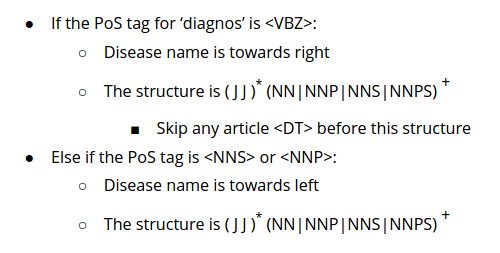
\includegraphics[width=3.2in]{img/rules.png}
\caption{Rules for word root 'diagnos'.}
\label{fig:rules}
\end{figure}


\subsubsection{Syntactic Constraints}

The syntactic constraint serves two purposes. First, it eliminates incoherent extractions, and second, it
reduces uninformative extractions by capturing relation phrases
expressed by only certain combinations. 

The reason for it being that entities in news headlines generally occur as the regular expression given below:

\[E = [DT][JJ]^*(NN|NNP|NNS|NNPS)^+\]

Or in other words, phrases that contain an optional determiner or article (e.g. a, an)  followed by multiple optional adjectives (e.g. fractured) and atleast one occurence of noun (e.g. elbow, non-Hodgskins lymphoma) with a maximum chain length of four. 
 
Since disease names basically represent a kind of entities, the above syntactic constraint extracts the potential disease name phrases from news headlines. For obvious reasons, we omit the determiner or article (represented by the PoS tag: DT), in order to get the disease names. For example, in the below headline: \\

\textit{Former Butler forward Andrew Smith \textbf{diagnosed with} non-Hodgskins lymphoma 
}\\

The extracted disease name is \textit{'non-Hodgskins lymphoma'}.


\subsubsection{Generalization}
Since a basic entity is represented by the regular expression discussed earlier, our SL-FII approach can be generalized for entities of other domains. This can be possible via simple modification of lexical constraints as per the context requirements. For example in order to identify the names of cricketers, we can use word roots like:

\begin{itemize}
\item 'wicket haul' derivatives
\item 'ton' derivatives
\end{itemize}

In the headlines below, we can successfully extract the cricketer's name using our SL-FII model.\\

\textit{Gayle's 47-ball \textbf{ton} wipes out England }

\textit{Ashwin's 5 \textbf{wicket haul} takes India to the semis}


\subsection{Frequency-based Iterative Improvement}

In this section, we describe the details of the Frequency-based Iterative Improvement (FII) phase. 
The constraints formulated above are then used to extract disease names from the corpus in an initial pass. Next, the potential disease names are passed through the FII phase.

Citations within the text should include the author's last name and
the year of publication, for example~\cite{gottlob:nonmon}.  Append
lowercase letters to the year in cases of ambiguity.  Treat multiple
authors as in the following examples:~\cite{abelson-et-al:scheme}
or~\cite{bgf:Lixto} (for more than two authors) and
\cite{brachman-schmolze:kl-one} (for two authors).  If the author
portion of a citation is obvious, omit it, e.g.,
Nebel~\shortcite{nebel:jair-2000}.  Collapse multiple citations as
follows:~\cite{gls:hypertrees,levesque:functional-foundations}.
\nocite{abelson-et-al:scheme}
\nocite{bgf:Lixto}
\nocite{brachman-schmolze:kl-one}
\nocite{gottlob:nonmon}
\nocite{gls:hypertrees}
\nocite{levesque:functional-foundations}
\nocite{levesque:belief}
\nocite{nebel:jair-2000}

\subsection{Footnotes}

Place footnotes at the bottom of the page in a 9-point font.  Refer to
them with superscript numbers.\footnote{This is how your footnotes
should appear.} Separate them from the text by a short
line.\footnote{Note the line separating these footnotes from the
text.} Avoid footnotes as much as possible; they interrupt the flow of
the text.

\section{Illustrations}

Place all illustrations (figures, drawings, tables, and photographs)
throughout the paper at the places where they are first discussed,
rather than at the end of the paper. If placed at the bottom or top of
a page, illustrations may run across both columns.

Illustrations must be rendered electronically or scanned and placed
directly in your document. All illustrations should be in black and
white, as color illustrations may cause problems. Line weights should
be 1/2-point or thicker. Avoid screens and superimposing type on
patterns as these effects may not reproduce well.

Number illustrations sequentially. Use references of the following
form: Figure 1, Table 2, etc. Place illustration numbers and captions
under illustrations. Leave a margin of 1/4-inch around the area
covered by the illustration and caption.  Use 9-point type for
captions, labels, and other text in illustrations.

\section*{Acknowledgments}

The preparation of these instructions and the \LaTeX{} and Bib\TeX{}
files that implement them was supported by Schlumberger Palo Alto
Research, AT\&T Bell Laboratories, and Morgan Kaufmann Publishers.
Preparation of the Microsoft Word file was supported by IJCAI.  An
early version of this document was created by Shirley Jowell and Peter
F. Patel-Schneider.  It was subsequently modified by Jennifer
Ballentine and Thomas Dean, Bernhard Nebel, and Daniel Pagenstecher.
These instructions are the same as the ones for IJCAI--05, prepared by
Kurt Steinkraus, Massachusetts Institute of Technology, Computer
Science and Artificial Intelligence Lab.

\appendix

\section{\LaTeX{} and Word Style Files}\label{stylefiles}

The \LaTeX{} and Word style files are available on the IJCAI--16
website, {\tt http://www.ijcai-16.org/}.
These style files implement the formatting instructions in this
document.

The \LaTeX{} files are {\tt ijcai16.sty} and {\tt ijcai16.tex}, and
the Bib\TeX{} files are {\tt named.bst} and {\tt ijcai16.bib}. The
\LaTeX{} style file is for version 2e of \LaTeX{}, and the Bib\TeX{}
style file is for version 0.99c of Bib\TeX{} ({\em not} version
0.98i). The {\tt ijcai16.sty} file is the same as the {\tt
ijcai07.sty} file used for IJCAI--07.

The Microsoft Word style file consists of a single file, {\tt
ijcai16.doc}. This template is the same as the one used for
IJCAI--07.

These Microsoft Word and \LaTeX{} files contain the source of the
present document and may serve as a formatting sample.  

Further information on using these styles for the preparation of
papers for IJCAI--16 can be obtained by contacting {\tt
ijcai16programchair@gmail.com}.

%% The file named.bst is a bibliography style file for BibTeX 0.99c
\bibliographystyle{named}
\bibliography{ijcai16}

\end{document}

